\documentclass{standalone}
\usepackage{tikz}
\usepackage{pgfplots}
\pgfplotsset{width=32cm,height=18cm,compat=1.3}
\pgfplotsset{every tick label/.append style={font=\Huge}}
\usepackage{filecontents}

\usetikzlibrary{patterns}

\definecolor{citrine}{rgb}{0.89, 0.82, 0.04}
\definecolor{arylideyellow}{rgb}{0.91, 0.84, 0.42}
\definecolor{bronze}{rgb}{0.8, 0.5, 0.2}

\begin{document}
	\centering
		\vspace{1.5em}
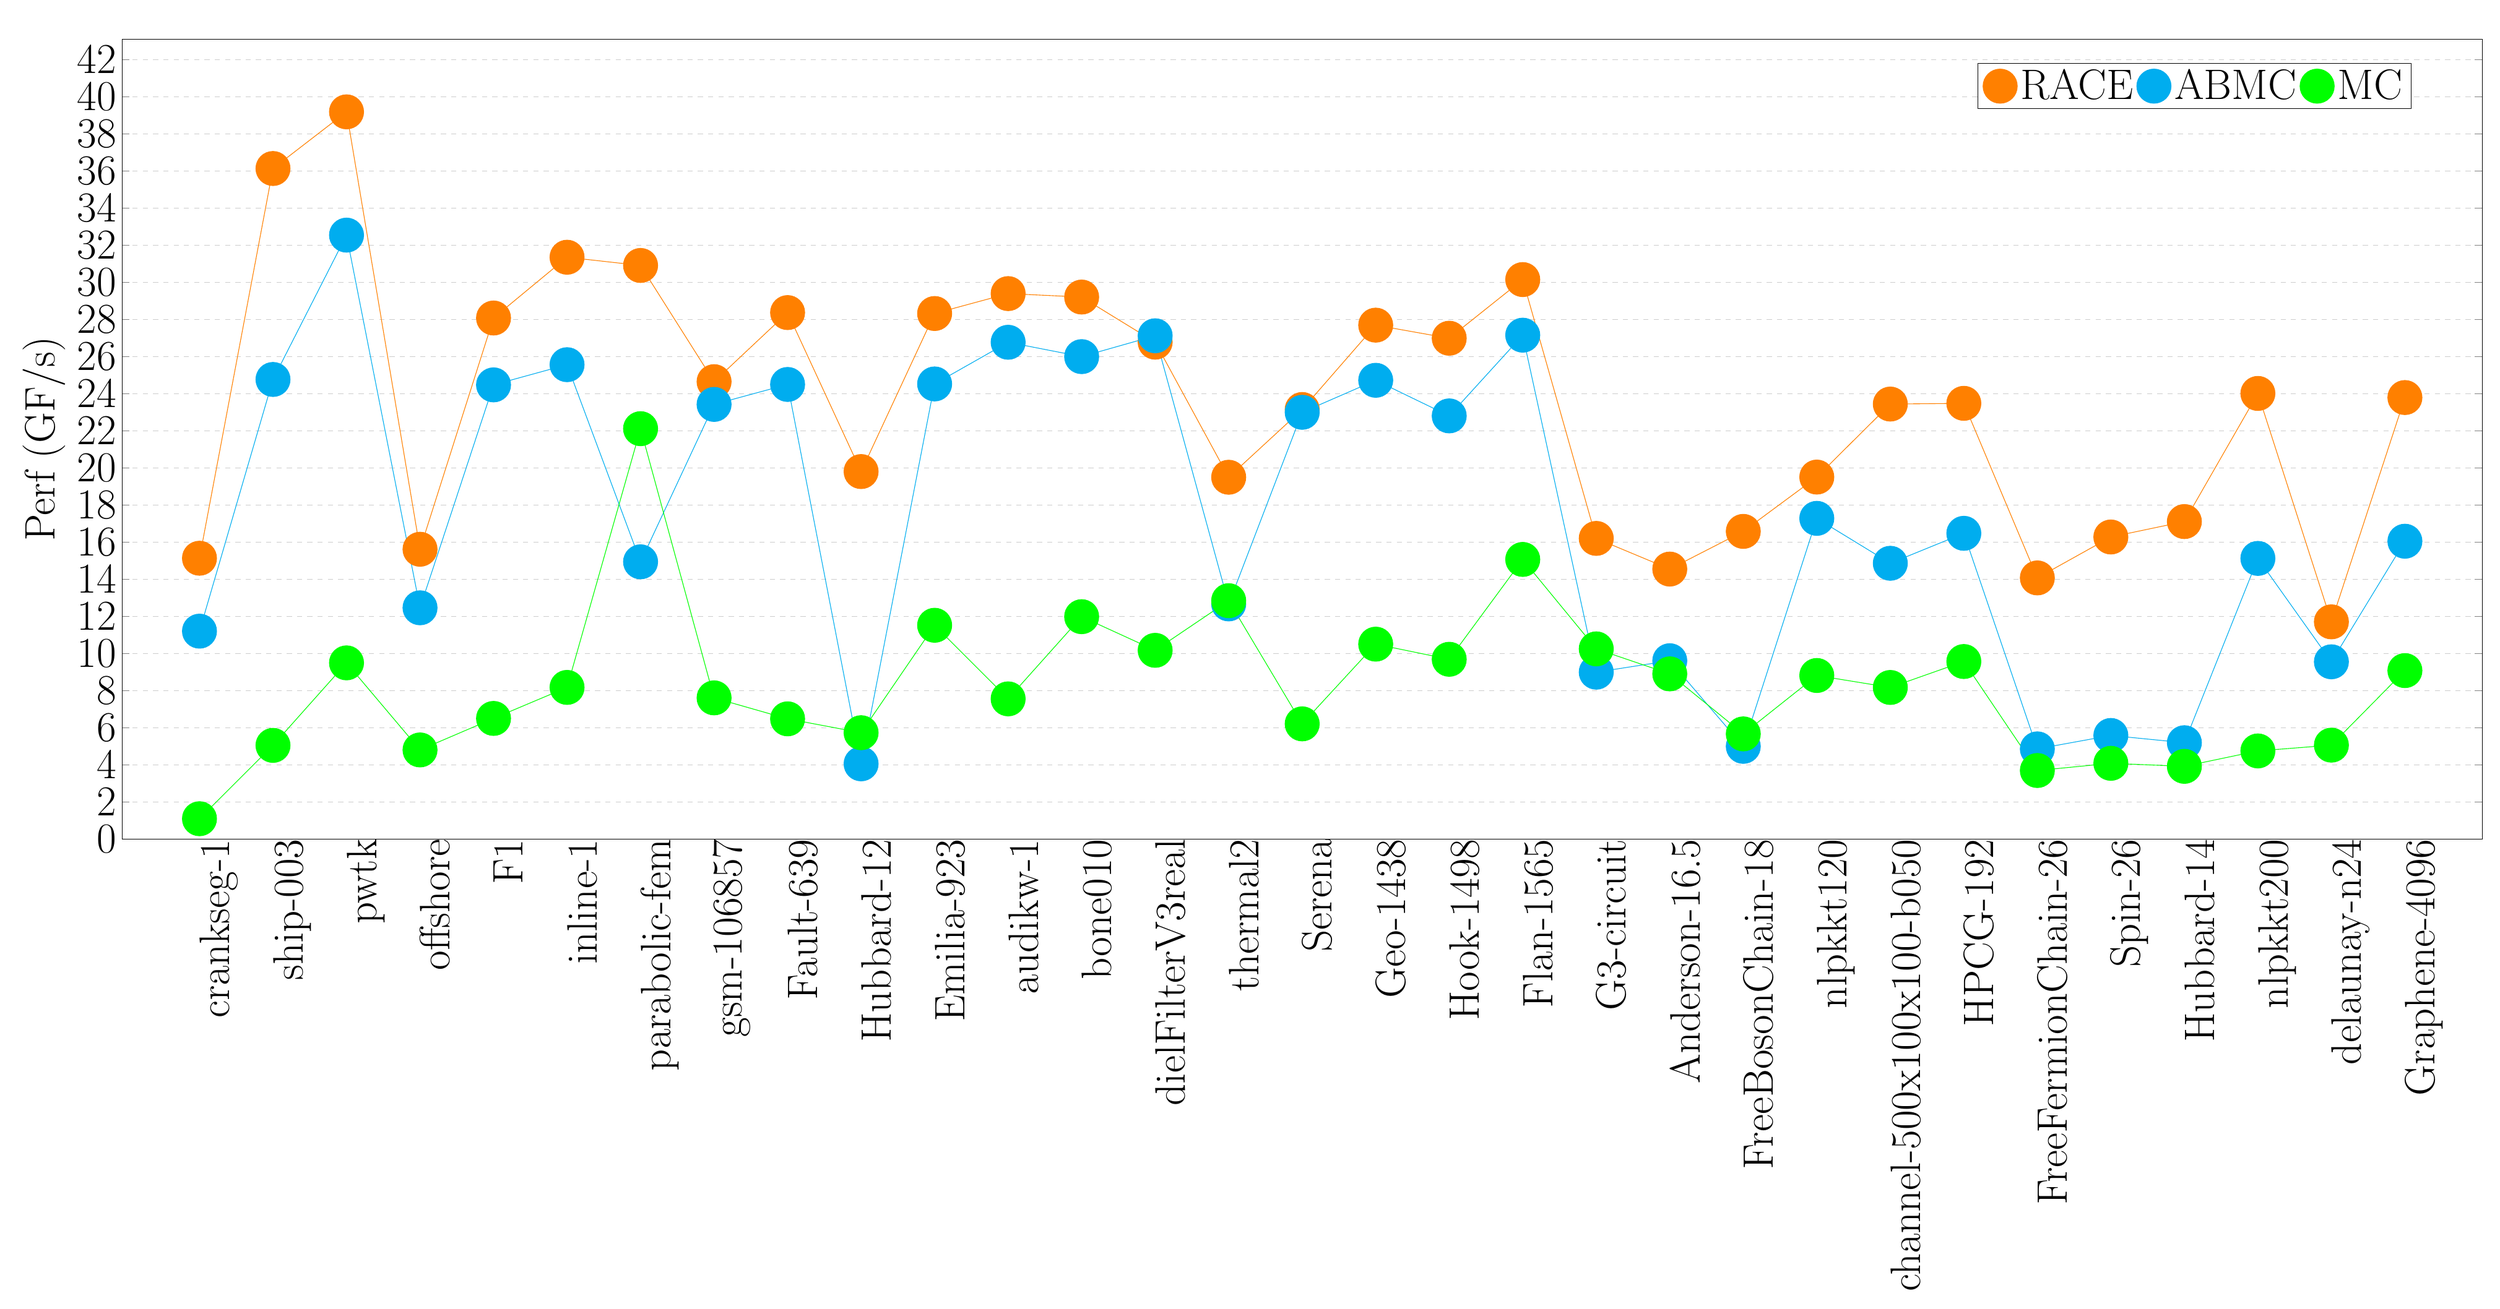
\begin{tikzpicture}
		%	\node at (13.25,15) {\LARGE{}};
			\begin{axis}[
		%	xmin=0.25, xmax=7.25,
			ymin=0, %ymax=3.25,
			xtick={1, 2, 3, 4, 5, 6, 7, 8, 9, 10, 11, 12, 13, 14, 15, 16, 17, 18, 19, 20, 21, 22, 23, 24, 25, 26, 27, 28, 29, 30, 31},
		%	ytick={0,0.5,1,1.5,2,2.5,3},
			xticklabels={crankseg-1, ship-003, pwtk, offshore, F1, inline-1, parabolic-fem, gsm-106857, Fault-639, Hubbard-12, Emilia-923, audikw-1, bone010, dielFilterV3real, thermal2, Serena, Geo-1438, Hook-1498, Flan-1565, G3-circuit, Anderson-16.5, FreeBosonChain-18, nlpkkt120, channel-500x100x100-b050, HPCG-192, FreeFermionChain-26, Spin-26, Hubbard-14, nlpkkt200, delaunay-n24, Graphene-4096},
			width  = 50cm,
			height = 18cm,
			major x tick style = transparent,
			%	minor ytick={1, 5, 10, 15, 20, 25, 30 ,35,40},
			grid = minor,	
			%add_bar_commands
			ymajorgrids = true,
			grid style={dashed, gray!40},
			ylabel = {\Huge{Perf (GF/s)}},
		%	symbolic x coords={Graphene-2048-2048, Graphene-4096-4096, Spin-24-24-24},
			x tick label style={rotate=90, anchor=north east, inner sep=0mm, font={\Huge}},
			tick label style={font={\Huge}},
			scaled y ticks = false,
			enlarge x limits=0.035,
			legend cell align=left,
			legend style={font=\Huge},
			legend columns=-1,
			legend style={
				%at={(1,1.05)},
				%anchor=south east,
				%column sep=1ex,
				legend pos=north east
			},
			%spl_legend_code
			title= {\Huge\scalebox{1.5}{{}}}
			]

\addplot[ mark=*, mark size=10pt, mark options={orange}, draw=orange ] plot coordinates{(1,15.130207) (2,36.140175) (3,39.194893) (4,15.613967) (5,28.080251) (6,31.356939) (7,30.913152) (8,24.649314) (9,28.372987) (10,19.802304) (11,28.323231) (12,29.396679) (13,29.210280) (14,26.778583) (15,19.496395) (16,23.148677) (17,27.696097) (18,26.990050) (19,30.152423) (20,16.199662) (21,14.545610) (22,16.577436) (23,19.505411) (24,23.441453) (25,23.480804) (26,14.069287) (27,16.275497) (28,17.107030) (29,24.014713) (30,11.700657) (31,23.793009)};
\addplot[ mark=*, mark size=10pt, mark options={cyan}, draw=cyan ] plot coordinates{(1,11.198986) (2,24.768035) (3,32.548921) (4,12.458177) (5,24.475683) (6,25.563859) (7,14.936887) (8,23.422725) (9,24.498829) (10,4.046577) (11,24.526497) (12,26.773144) (13,25.998597) (14,27.122656) (15,12.667727) (16,22.996604) (17,24.722981) (18,22.803733) (19,27.155631) (20,8.987108) (21,9.605270) (22,4.988385) (23,17.279764) (24,14.858202) (25,16.473370) (26,4.853501) (27,5.575532) (28,5.185500) (29,15.120960) (30,9.546883) (31,16.047102)};
\addplot[ mark=*, mark size=10pt, mark options={green}, draw=green ] plot coordinates{(1,1.087234) (2,5.041221) (3,9.489892) (4,4.795549) (5,6.494727) (6,8.166534) (7,22.114680) (8,7.603073) (9,6.471868) (10,5.724418) (11,11.516064) (12,7.549159) (13,11.979405) (14,10.165285) (15,12.841705) (16,6.201050) (17,10.498566) (18,9.682819) (19,15.065381) (20,10.243942) (21,8.895866) (22,5.660339) (23,8.808741) (24,8.163804) (25,9.562151) (26,3.686573) (27,4.074622) (28,3.911298) (29,4.742299) (30,5.053941) (31,9.073864)};
	%addplot cmd

	\legend{RACE, ABMC, MC}

	\end{axis}			
\end{tikzpicture}

\end{document}

